\documentclass[1p]{elsarticle_modified}
%\bibliographystyle{elsarticle-num}

%\usepackage[colorlinks]{hyperref}
%\usepackage{abbrmath_seonhwa} %\Abb, \Ascr, \Acal ,\Abf, \Afrak
\usepackage{amsfonts}
\usepackage{amssymb}
\usepackage{amsmath}
\usepackage{amsthm}
\usepackage{scalefnt}
\usepackage{amsbsy}
\usepackage{kotex}
\usepackage{caption}
\usepackage{subfig}
\usepackage{color}
\usepackage{graphicx}
\usepackage{xcolor} %% white, black, red, green, blue, cyan, magenta, yellow
\usepackage{float}
\usepackage{setspace}
\usepackage{hyperref}

\usepackage{tikz}
\usetikzlibrary{arrows}

\usepackage{multirow}
\usepackage{array} % fixed length table
\usepackage{hhline}

%%%%%%%%%%%%%%%%%%%%%
\makeatletter
\renewcommand*\env@matrix[1][\arraystretch]{%
	\edef\arraystretch{#1}%
	\hskip -\arraycolsep
	\let\@ifnextchar\new@ifnextchar
	\array{*\c@MaxMatrixCols c}}
\makeatother %https://tex.stackexchange.com/questions/14071/how-can-i-increase-the-line-spacing-in-a-matrix
%%%%%%%%%%%%%%%

\usepackage[normalem]{ulem}

\newcommand{\msout}[1]{\ifmmode\text{\sout{\ensuremath{#1}}}\else\sout{#1}\fi}
%SOURCE: \msout is \stkout macro in https://tex.stackexchange.com/questions/20609/strikeout-in-math-mode

\newcommand{\cancel}[1]{
	\ifmmode
	{\color{red}\msout{#1}}
	\else
	{\color{red}\sout{#1}}
	\fi
}

\newcommand{\add}[1]{
	{\color{blue}\uwave{#1}}
}

\newcommand{\replace}[2]{
	\ifmmode
	{\color{red}\msout{#1}}{\color{blue}\uwave{#2}}
	\else
	{\color{red}\sout{#1}}{\color{blue}\uwave{#2}}
	\fi
}

\newcommand{\Sol}{\mathcal{S}} %segment
\newcommand{\D}{D} %diagram
\newcommand{\A}{\mathcal{A}} %arc


%%%%%%%%%%%%%%%%%%%%%%%%%%%%%5 test

\def\sl{\operatorname{\textup{SL}}(2,\Cbb)}
\def\psl{\operatorname{\textup{PSL}}(2,\Cbb)}
\def\quan{\mkern 1mu \triangleright \mkern 1mu}

\theoremstyle{definition}
\newtheorem{thm}{Theorem}[section]
\newtheorem{prop}[thm]{Proposition}
\newtheorem{lem}[thm]{Lemma}
\newtheorem{ques}[thm]{Question}
\newtheorem{cor}[thm]{Corollary}
\newtheorem{defn}[thm]{Definition}
\newtheorem{exam}[thm]{Example}
\newtheorem{rmk}[thm]{Remark}
\newtheorem{alg}[thm]{Algorithm}

\newcommand{\I}{\sqrt{-1}}
\begin{document}

%\begin{frontmatter}
%
%\title{Boundary parabolic representations of knots up to 8 crossings}
%
%%% Group authors per affiliation:
%\author{Yunhi Cho} 
%\address{Department of Mathematics, University of Seoul, Seoul, Korea}
%\ead{yhcho@uos.ac.kr}
%
%
%\author{Seonhwa Kim} %\fnref{s_kim}}
%\address{Center for Geometry and Physics, Institute for Basic Science, Pohang, 37673, Korea}
%\ead{ryeona17@ibs.re.kr}
%
%\author{Hyuk Kim}
%\address{Department of Mathematical Sciences, Seoul National University, Seoul 08826, Korea}
%\ead{hyukkim@snu.ac.kr}
%
%\author{Seokbeom Yoon}
%\address{Department of Mathematical Sciences, Seoul National University, Seoul, 08826,  Korea}
%\ead{sbyoon15@snu.ac.kr}
%
%\begin{abstract}
%We find all boundary parabolic representation of knots up to 8 crossings.
%
%\end{abstract}
%\begin{keyword}
%    \MSC[2010] 57M25 
%\end{keyword}
%
%\end{frontmatter}

%\linenumbers
%\tableofcontents
%
\newcommand\colored[1]{\textcolor{white}{\rule[-0.35ex]{0.8em}{1.4ex}}\kern-0.8em\color{red} #1}%
%\newcommand\colored[1]{\textcolor{white}{ #1}\kern-2.17ex	\textcolor{white}{ #1}\kern-1.81ex	\textcolor{white}{ #1}\kern-2.15ex\color{red}#1	}

{\Large $\underline{12a_{1035}~(K12a_{1035})}$}

\setlength{\tabcolsep}{10pt}
\renewcommand{\arraystretch}{1.6}
\vspace{1cm}\begin{tabular}{m{100pt}>{\centering\arraybackslash}m{274pt}}
\multirow{5}{120pt}{
	\centering
	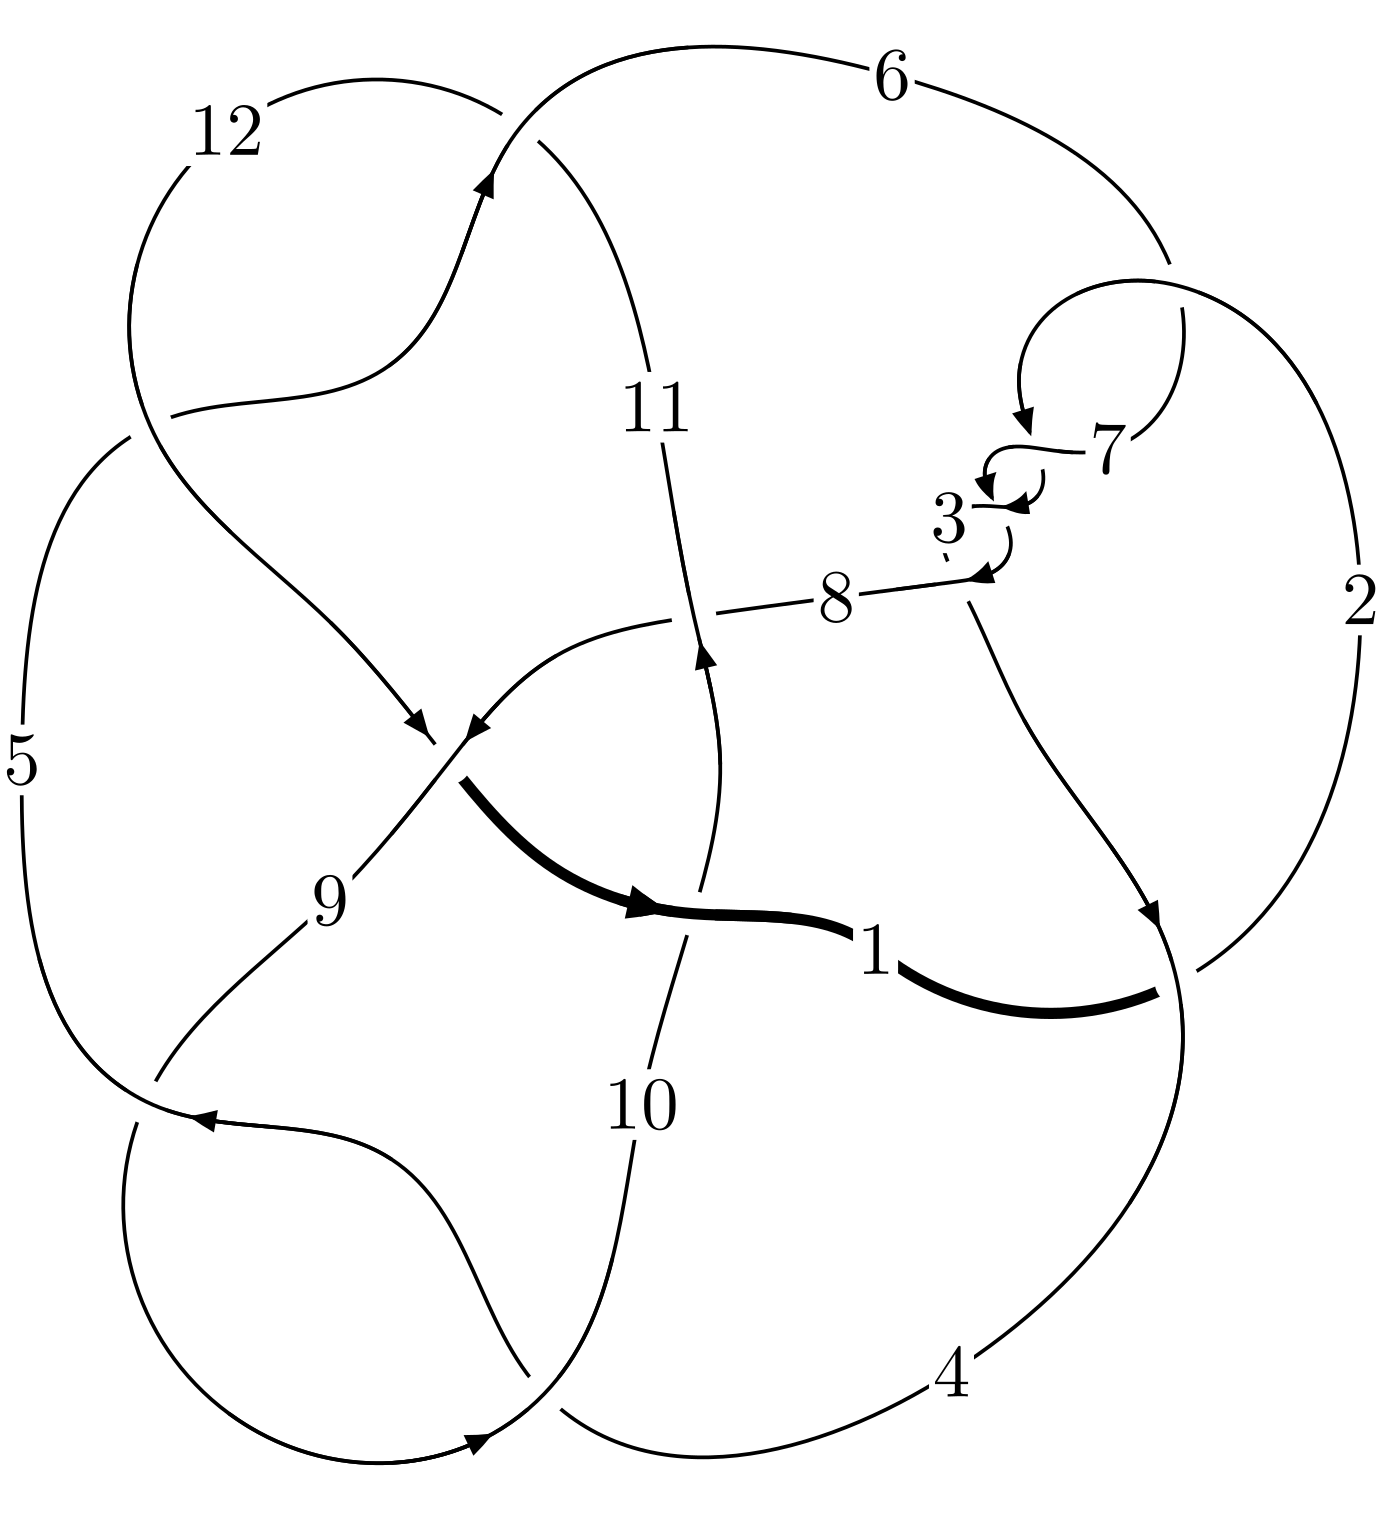
\includegraphics[width=112pt]{../../../GIT/diagram.site/Diagrams/png/1836_12a_1035.png}\\
\ \ \ A knot diagram\footnotemark}&
\allowdisplaybreaks
\textbf{Linearized knot diagam} \\
\cline{2-2}
 &
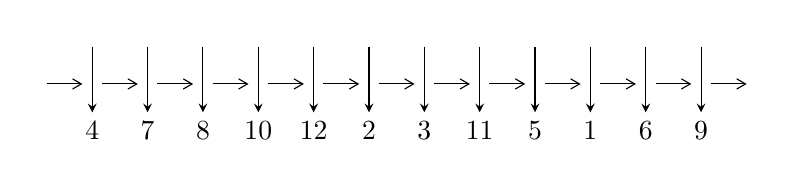
\begin{tikzpicture}[x=20pt, y=17pt]
	% nodes
	\node (C0) at (0, 0) {};
	\node (C1) at (1, 0) {};
	\node (C1U) at (1, +1) {};
	\node (C1D) at (1, -1) {4};

	\node (C2) at (2, 0) {};
	\node (C2U) at (2, +1) {};
	\node (C2D) at (2, -1) {7};

	\node (C3) at (3, 0) {};
	\node (C3U) at (3, +1) {};
	\node (C3D) at (3, -1) {8};

	\node (C4) at (4, 0) {};
	\node (C4U) at (4, +1) {};
	\node (C4D) at (4, -1) {10};

	\node (C5) at (5, 0) {};
	\node (C5U) at (5, +1) {};
	\node (C5D) at (5, -1) {12};

	\node (C6) at (6, 0) {};
	\node (C6U) at (6, +1) {};
	\node (C6D) at (6, -1) {2};

	\node (C7) at (7, 0) {};
	\node (C7U) at (7, +1) {};
	\node (C7D) at (7, -1) {3};

	\node (C8) at (8, 0) {};
	\node (C8U) at (8, +1) {};
	\node (C8D) at (8, -1) {11};

	\node (C9) at (9, 0) {};
	\node (C9U) at (9, +1) {};
	\node (C9D) at (9, -1) {5};

	\node (C10) at (10, 0) {};
	\node (C10U) at (10, +1) {};
	\node (C10D) at (10, -1) {1};

	\node (C11) at (11, 0) {};
	\node (C11U) at (11, +1) {};
	\node (C11D) at (11, -1) {6};

	\node (C12) at (12, 0) {};
	\node (C12U) at (12, +1) {};
	\node (C12D) at (12, -1) {9};
	\node (C13) at (13, 0) {};

	% arrows
	\draw[->,>={angle 60}]
	(C0) edge (C1) (C1) edge (C2) (C2) edge (C3) (C3) edge (C4) (C4) edge (C5) (C5) edge (C6) (C6) edge (C7) (C7) edge (C8) (C8) edge (C9) (C9) edge (C10) (C10) edge (C11) (C11) edge (C12) (C12) edge (C13) ;	\draw[->,>=stealth]
	(C1U) edge (C1D) (C2U) edge (C2D) (C3U) edge (C3D) (C4U) edge (C4D) (C5U) edge (C5D) (C6U) edge (C6D) (C7U) edge (C7D) (C8U) edge (C8D) (C9U) edge (C9D) (C10U) edge (C10D) (C11U) edge (C11D) (C12U) edge (C12D) ;
	\end{tikzpicture} \\
\hhline{~~} \\& 
\textbf{Solving Sequence} \\ \cline{2-2} 
 &
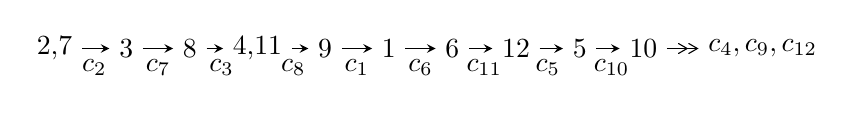
\begin{tikzpicture}[x=23pt, y=7pt]
	% node
	\node (A0) at (-1/8, 0) {2,7};
	\node (A1) at (1, 0) {3};
	\node (A2) at (2, 0) {8};
	\node (A3) at (49/16, 0) {4,11};
	\node (A4) at (33/8, 0) {9};
	\node (A5) at (41/8, 0) {1};
	\node (A6) at (49/8, 0) {6};
	\node (A7) at (57/8, 0) {12};
	\node (A8) at (65/8, 0) {5};
	\node (A9) at (73/8, 0) {10};
	\node (C1) at (1/2, -1) {$c_{2}$};
	\node (C2) at (3/2, -1) {$c_{7}$};
	\node (C3) at (5/2, -1) {$c_{3}$};
	\node (C4) at (29/8, -1) {$c_{8}$};
	\node (C5) at (37/8, -1) {$c_{1}$};
	\node (C6) at (45/8, -1) {$c_{6}$};
	\node (C7) at (53/8, -1) {$c_{11}$};
	\node (C8) at (61/8, -1) {$c_{5}$};
	\node (C9) at (69/8, -1) {$c_{10}$};
	\node (A10) at (11, 0) {$c_{4},c_{9},c_{12}$};

	% edge
	\draw[->,>=stealth]	
	(A0) edge (A1) (A1) edge (A2) (A2) edge (A3) (A3) edge (A4) (A4) edge (A5) (A5) edge (A6) (A6) edge (A7) (A7) edge (A8) (A8) edge (A9) ;
	\draw[->>,>={angle 60}]	
	(A9) edge (A10);
\end{tikzpicture} \\ 

\end{tabular} \\

\footnotetext{
The image of knot diagram is generated by the software ``\textbf{Draw programme}" developed by Andrew Bartholomew(\url{http://www.layer8.co.uk/maths/draw/index.htm\#Running-draw}), where we modified some parts for our purpose(\url{https://github.com/CATsTAILs/LinksPainter}).
}\phantom \\ \newline 
\centering \textbf{Ideals for irreducible components\footnotemark of $X_{\text{par}}$} 
 
\begin{align*}
I^u_{1}&=\langle 
-181 u^{30}-802 u^{29}+\cdots+2 b+456,\;-133 u^{30}-587 u^{29}+\cdots+2 a+329,\;u^{31}+6 u^{30}+\cdots+14 u-4\rangle \\
I^u_{2}&=\langle 
22271 u^{14} a^3-122677 u^{14} a^2+\cdots+165657 a-109901,\;- u^{14} a^2+7 u^{14} a+\cdots-30 a+28,\\
\phantom{I^u_{2}}&\phantom{= \langle  }u^{15}- u^{14}-8 u^{13}+7 u^{12}+24 u^{11}-16 u^{10}-34 u^9+11 u^8+26 u^7+2 u^6-14 u^5+4 u^3+2 u^2-2 u-1\rangle \\
I^u_{3}&=\langle 
- u^{13}+7 u^{11}+u^{10}-17 u^9-4 u^8+16 u^7+2 u^6-7 u^5+5 u^4+7 u^3- u^2+b,\\
\phantom{I^u_{3}}&\phantom{= \langle  }- u^{12}+8 u^{10}-22 u^8+24 u^6-2 u^5-11 u^4+6 u^3+7 u^2+a-3 u,\\
\phantom{I^u_{3}}&\phantom{= \langle  }u^{14}- u^{13}-8 u^{12}+7 u^{11}+24 u^{10}-17 u^9-33 u^8+17 u^7+21 u^6-10 u^5-7 u^4+9 u^3+2 u^2- u-1\rangle \\
\\
\end{align*}
\raggedright * 3 irreducible components of $\dim_{\mathbb{C}}=0$, with total 105 representations.\\
\footnotetext{All coefficients of polynomials are rational numbers. But the coefficients are sometimes approximated in decimal forms when there is not enough margin.}
\newpage
\renewcommand{\arraystretch}{1}
\centering \section*{I. $I^u_{1}= \langle -181 u^{30}-802 u^{29}+\cdots+2 b+456,\;-133 u^{30}-587 u^{29}+\cdots+2 a+329,\;u^{31}+6 u^{30}+\cdots+14 u-4 \rangle$}
\flushleft \textbf{(i) Arc colorings}\\
\begin{tabular}{m{7pt} m{180pt} m{7pt} m{180pt} }
\flushright $a_{2}=$&$\begin{pmatrix}1\\0\end{pmatrix}$ \\
\flushright $a_{7}=$&$\begin{pmatrix}0\\u\end{pmatrix}$ \\
\flushright $a_{3}=$&$\begin{pmatrix}1\\u^2\end{pmatrix}$ \\
\flushright $a_{8}=$&$\begin{pmatrix}- u\\- u^3+u\end{pmatrix}$ \\
\flushright $a_{4}=$&$\begin{pmatrix}- u^2+1\\- u^4+2 u^2\end{pmatrix}$ \\
\flushright $a_{11}=$&$\begin{pmatrix}\frac{133}{2} u^{30}+\frac{587}{2} u^{29}+\cdots+686 u-\frac{329}{2}\\\frac{181}{2} u^{30}+401 u^{29}+\cdots+\frac{1881}{2} u-228\end{pmatrix}$ \\
\flushright $a_{9}=$&$\begin{pmatrix}-\frac{79}{4} u^{30}-89 u^{29}+\cdots-\frac{885}{4} u+52\\-\frac{59}{2} u^{30}-132 u^{29}+\cdots-\frac{639}{2} u+77\end{pmatrix}$ \\
\flushright $a_{1}=$&$\begin{pmatrix}- u^6+3 u^4-2 u^2+1\\- u^8+4 u^6-4 u^4\end{pmatrix}$ \\
\flushright $a_{6}=$&$\begin{pmatrix}u\\u\end{pmatrix}$ \\
\flushright $a_{12}=$&$\begin{pmatrix}\frac{21}{2} u^{30}+\frac{83}{2} u^{29}+\cdots+79 u-\frac{37}{2}\\\frac{69}{2} u^{30}+149 u^{29}+\cdots+\frac{667}{2} u-82\end{pmatrix}$ \\
\flushright $a_{5}=$&$\begin{pmatrix}-\frac{49}{4} u^{30}-54 u^{29}+\cdots-\frac{479}{4} u+30\\-\frac{21}{2} u^{30}-48 u^{29}+\cdots-\frac{241}{2} u+29\end{pmatrix}$ \\
\flushright $a_{10}=$&$\begin{pmatrix}- u^{30}+\frac{1}{2} u^{29}+\cdots+\frac{57}{2} u-\frac{9}{2}\\\frac{7}{2} u^{30}+20 u^{29}+\cdots+\frac{141}{2} u-16\end{pmatrix}$\\&\end{tabular}
\flushleft \textbf{(ii) Obstruction class $= -1$}\\~\\
\flushleft \textbf{(iii) Cusp Shapes $= -81 u^{30}-353 u^{29}+499 u^{28}+3872 u^{27}-74 u^{26}-17898 u^{25}-4528 u^{24}+48948 u^{23}+3960 u^{22}-97075 u^{21}+31813 u^{20}+144406 u^{19}-112024 u^{18}-128297 u^{17}+202242 u^{16}+19409 u^{15}-222196 u^{14}+102946 u^{13}+118470 u^{12}-155647 u^{11}-3449 u^{10}+92237 u^9-51860 u^8-22781 u^7+31120 u^6-7025 u^5-7682 u^4+4279 u^3-14 u^2-756 u+170$}\\~\\
\newpage\renewcommand{\arraystretch}{1}
\flushleft \textbf{(iv) u-Polynomials at the component}\newline \\
\begin{tabular}{m{50pt}|m{274pt}}
Crossings & \hspace{64pt}u-Polynomials at each crossing \\
\hline $$\begin{aligned}c_{1}\end{aligned}$$&$\begin{aligned}
&u^{31}-6 u^{30}+\cdots+17032 u+3008
\end{aligned}$\\
\hline $$\begin{aligned}c_{2},c_{3},c_{6}\\c_{7}\end{aligned}$$&$\begin{aligned}
&u^{31}-6 u^{30}+\cdots+14 u+4
\end{aligned}$\\
\hline $$\begin{aligned}c_{4},c_{5},c_{9}\\c_{11}\end{aligned}$$&$\begin{aligned}
&u^{31}+12 u^{29}+\cdots+2 u+1
\end{aligned}$\\
\hline $$\begin{aligned}c_{8},c_{10}\end{aligned}$$&$\begin{aligned}
&u^{31}+2 u^{30}+\cdots+11 u+1
\end{aligned}$\\
\hline $$\begin{aligned}c_{12}\end{aligned}$$&$\begin{aligned}
&u^{31}+33 u^{30}+\cdots+655360 u+32768
\end{aligned}$\\
\hline
\end{tabular}\\~\\
\newpage\renewcommand{\arraystretch}{1}
\flushleft \textbf{(v) Riley Polynomials at the component}\newline \\
\begin{tabular}{m{50pt}|m{274pt}}
Crossings & \hspace{64pt}Riley Polynomials at each crossing \\
\hline $$\begin{aligned}c_{1}\end{aligned}$$&$\begin{aligned}
&y^{31}+14 y^{30}+\cdots+194260160 y-9048064
\end{aligned}$\\
\hline $$\begin{aligned}c_{2},c_{3},c_{6}\\c_{7}\end{aligned}$$&$\begin{aligned}
&y^{31}-34 y^{30}+\cdots+268 y-16
\end{aligned}$\\
\hline $$\begin{aligned}c_{4},c_{5},c_{9}\\c_{11}\end{aligned}$$&$\begin{aligned}
&y^{31}+24 y^{30}+\cdots+12 y-1
\end{aligned}$\\
\hline $$\begin{aligned}c_{8},c_{10}\end{aligned}$$&$\begin{aligned}
&y^{31}+2 y^{30}+\cdots+29 y-1
\end{aligned}$\\
\hline $$\begin{aligned}c_{12}\end{aligned}$$&$\begin{aligned}
&y^{31}+3 y^{30}+\cdots+20401094656 y-1073741824
\end{aligned}$\\
\hline
\end{tabular}\\~\\
\newpage\flushleft \textbf{(vi) Complex Volumes and Cusp Shapes}
$$\begin{array}{c|c|c}  
\text{Solutions to }I^u_{1}& \I (\text{vol} + \sqrt{-1}CS) & \text{Cusp shape}\\
 \hline 
\begin{aligned}
u &= \phantom{-}0.689568 + 0.711824 I \\
a &= \phantom{-}0.130088 - 0.331811 I \\
b &= \phantom{-}1.002630 + 0.498746 I\end{aligned}
 & \phantom{-}5.82989 - 3.44362 I & -5.04834 + 9.30785 I \\ \hline\begin{aligned}
u &= \phantom{-}0.689568 - 0.711824 I \\
a &= \phantom{-}0.130088 + 0.331811 I \\
b &= \phantom{-}1.002630 - 0.498746 I\end{aligned}
 & \phantom{-}5.82989 + 3.44362 I & -5.04834 - 9.30785 I \\ \hline\begin{aligned}
u &= \phantom{-}0.644371 + 0.613769 I \\
a &= -0.242643 + 0.183681 I \\
b &= -1.78223 - 0.62081 I\end{aligned}
 & \phantom{-}8.1222 - 13.5080 I & -8.59420 + 9.11815 I \\ \hline\begin{aligned}
u &= \phantom{-}0.644371 - 0.613769 I \\
a &= -0.242643 - 0.183681 I \\
b &= -1.78223 + 0.62081 I\end{aligned}
 & \phantom{-}8.1222 + 13.5080 I & -8.59420 - 9.11815 I \\ \hline\begin{aligned}
u &= -1.052860 + 0.374486 I \\
a &= \phantom{-}0.147933 + 0.319672 I \\
b &= \phantom{-}0.749156 - 0.604636 I\end{aligned}
 & \phantom{-}2.99598 + 5.86638 I & -8.62905 - 10.38587 I \\ \hline\begin{aligned}
u &= -1.052860 - 0.374486 I \\
a &= \phantom{-}0.147933 - 0.319672 I \\
b &= \phantom{-}0.749156 + 0.604636 I\end{aligned}
 & \phantom{-}2.99598 - 5.86638 I & -8.62905 + 10.38587 I \\ \hline\begin{aligned}
u &= \phantom{-}0.246593 + 0.835945 I \\
a &= -0.706404 - 0.362266 I \\
b &= \phantom{-}0.645159 - 0.082571 I\end{aligned}
 & \phantom{-}7.12015 - 1.65223 I & \phantom{-}4.05704 + 1.14509 I \\ \hline\begin{aligned}
u &= \phantom{-}0.246593 - 0.835945 I \\
a &= -0.706404 + 0.362266 I \\
b &= \phantom{-}0.645159 + 0.082571 I\end{aligned}
 & \phantom{-}7.12015 + 1.65223 I & \phantom{-}4.05704 - 1.14509 I \\ \hline\begin{aligned}
u &= \phantom{-}0.326413 + 0.688470 I \\
a &= \phantom{-}0.76255 + 1.47066 I \\
b &= -0.692232 + 0.121974 I\end{aligned}
 & \phantom{-}9.06712 + 9.13286 I & -6.46930 - 3.89273 I \\ \hline\begin{aligned}
u &= \phantom{-}0.326413 - 0.688470 I \\
a &= \phantom{-}0.76255 - 1.47066 I \\
b &= -0.692232 - 0.121974 I\end{aligned}
 & \phantom{-}9.06712 - 9.13286 I & -6.46930 + 3.89273 I\\
 \hline 
 \end{array}$$\newpage$$\begin{array}{c|c|c}  
\text{Solutions to }I^u_{1}& \I (\text{vol} + \sqrt{-1}CS) & \text{Cusp shape}\\
 \hline 
\begin{aligned}
u &= \phantom{-}0.561340 + 0.467670 I \\
a &= \phantom{-}0.213153 + 0.590915 I \\
b &= \phantom{-}0.929737 - 0.172994 I\end{aligned}
 & -0.79381 - 3.44032 I & -15.0997 + 6.5409 I \\ \hline\begin{aligned}
u &= \phantom{-}0.561340 - 0.467670 I \\
a &= \phantom{-}0.213153 - 0.590915 I \\
b &= \phantom{-}0.929737 + 0.172994 I\end{aligned}
 & -0.79381 + 3.44032 I & -15.0997 - 6.5409 I \\ \hline\begin{aligned}
u &= -1.322110 + 0.192020 I \\
a &= -0.001468 - 0.451220 I \\
b &= \phantom{-}0.130828 + 0.618327 I\end{aligned}
 & \phantom{-}3.87543 - 5.94393 I & -9.66825 + 3.93876 I \\ \hline\begin{aligned}
u &= -1.322110 - 0.192020 I \\
a &= -0.001468 + 0.451220 I \\
b &= \phantom{-}0.130828 - 0.618327 I\end{aligned}
 & \phantom{-}3.87543 + 5.94393 I & -9.66825 - 3.93876 I \\ \hline\begin{aligned}
u &= -0.590937 + 0.161479 I \\
a &= -0.626188 - 0.664332 I \\
b &= -1.351820 - 0.247148 I\end{aligned}
 & -2.73754 + 0.38412 I & -17.5394 - 12.3371 I \\ \hline\begin{aligned}
u &= -0.590937 - 0.161479 I \\
a &= -0.626188 + 0.664332 I \\
b &= -1.351820 + 0.247148 I\end{aligned}
 & -2.73754 - 0.38412 I & -17.5394 + 12.3371 I \\ \hline\begin{aligned}
u &= \phantom{-}0.380886 + 0.410622 I \\
a &= \phantom{-}0.376186 - 0.990063 I \\
b &= -0.338423 - 0.093255 I\end{aligned}
 & -0.260092 + 0.248902 I & -13.42836 + 0.35598 I \\ \hline\begin{aligned}
u &= \phantom{-}0.380886 - 0.410622 I \\
a &= \phantom{-}0.376186 + 0.990063 I \\
b &= -0.338423 + 0.093255 I\end{aligned}
 & -0.260092 - 0.248902 I & -13.42836 - 0.35598 I \\ \hline\begin{aligned}
u &= -1.54304 + 0.09101 I \\
a &= -1.153730 - 0.253473 I \\
b &= -1.60000 - 0.46649 I\end{aligned}
 & -6.90265 + 1.26668 I & \phantom{-0.000000 } 0 \\ \hline\begin{aligned}
u &= -1.54304 - 0.09101 I \\
a &= -1.153730 + 0.253473 I \\
b &= -1.60000 + 0.46649 I\end{aligned}
 & -6.90265 - 1.26668 I & \phantom{-0.000000 } 0\\
 \hline 
 \end{array}$$\newpage$$\begin{array}{c|c|c}  
\text{Solutions to }I^u_{1}& \I (\text{vol} + \sqrt{-1}CS) & \text{Cusp shape}\\
 \hline 
\begin{aligned}
u &= -1.55633 + 0.13225 I \\
a &= \phantom{-}1.87141 + 0.87299 I \\
b &= \phantom{-}2.39850 + 1.02474 I\end{aligned}
 & -7.92003 + 5.59839 I & \phantom{-0.000000 } 0 \\ \hline\begin{aligned}
u &= -1.55633 - 0.13225 I \\
a &= \phantom{-}1.87141 - 0.87299 I \\
b &= \phantom{-}2.39850 - 1.02474 I\end{aligned}
 & -7.92003 - 5.59839 I & \phantom{-0.000000 } 0 \\ \hline\begin{aligned}
u &= \phantom{-}1.57004 + 0.04724 I \\
a &= -2.37428 + 0.51267 I \\
b &= -2.70859 + 0.17576 I\end{aligned}
 & -10.13910 - 1.16704 I & \phantom{-0.000000 } 0 \\ \hline\begin{aligned}
u &= \phantom{-}1.57004 - 0.04724 I \\
a &= -2.37428 - 0.51267 I \\
b &= -2.70859 - 0.17576 I\end{aligned}
 & -10.13910 + 1.16704 I & \phantom{-0.000000 } 0 \\ \hline\begin{aligned}
u &= -1.58052 + 0.19018 I \\
a &= -2.71394 - 0.04037 I \\
b &= -3.15957 + 0.84008 I\end{aligned}
 & \phantom{-}0.6908 + 16.4865 I & \phantom{-0.000000 } 0 \\ \hline\begin{aligned}
u &= -1.58052 - 0.19018 I \\
a &= -2.71394 + 0.04037 I \\
b &= -3.15957 - 0.84008 I\end{aligned}
 & \phantom{-}0.6908 - 16.4865 I & \phantom{-0.000000 } 0 \\ \hline\begin{aligned}
u &= -1.58443 + 0.22713 I \\
a &= \phantom{-}1.47735 + 0.07070 I \\
b &= \phantom{-}1.64032 - 0.65576 I\end{aligned}
 & -1.67379 + 6.94665 I & \phantom{-0.000000 } 0 \\ \hline\begin{aligned}
u &= -1.58443 - 0.22713 I \\
a &= \phantom{-}1.47735 - 0.07070 I \\
b &= \phantom{-}1.64032 + 0.65576 I\end{aligned}
 & -1.67379 - 6.94665 I & \phantom{-0.000000 } 0 \\ \hline\begin{aligned}
u &= \phantom{-}1.64692 + 0.06572 I \\
a &= \phantom{-}1.42991 + 0.89247 I \\
b &= \phantom{-}1.75616 + 1.56825 I\end{aligned}
 & -6.18258 - 7.30230 I & \phantom{-0.000000 } 0 \\ \hline\begin{aligned}
u &= \phantom{-}1.64692 - 0.06572 I \\
a &= \phantom{-}1.42991 - 0.89247 I \\
b &= \phantom{-}1.75616 - 1.56825 I\end{aligned}
 & -6.18258 + 7.30230 I & \phantom{-0.000000 } 0\\
 \hline 
 \end{array}$$\newpage$$\begin{array}{c|c|c}  
\text{Solutions to }I^u_{1}& \I (\text{vol} + \sqrt{-1}CS) & \text{Cusp shape}\\
 \hline 
\begin{aligned}
u &= \phantom{-}0.328219\phantom{ +0.000000I} \\
a &= \phantom{-}0.820145\phantom{ +0.000000I} \\
b &= -0.239259\phantom{ +0.000000I}\end{aligned}
 & -0.539109\phantom{ +0.000000I} & -18.1900\phantom{ +0.000000I}\\
 \hline 
 \end{array}$$\newpage\newpage\renewcommand{\arraystretch}{1}
\centering \section*{II. $I^u_{2}= \langle 2.23\times10^{4} a^{3} u^{14}-1.23\times10^{5} a^{2} u^{14}+\cdots+1.66\times10^{5} a-1.10\times10^{5},\;- u^{14} a^2+7 u^{14} a+\cdots-30 a+28,\;u^{15}- u^{14}+\cdots-2 u-1 \rangle$}
\flushleft \textbf{(i) Arc colorings}\\
\begin{tabular}{m{7pt} m{180pt} m{7pt} m{180pt} }
\flushright $a_{2}=$&$\begin{pmatrix}1\\0\end{pmatrix}$ \\
\flushright $a_{7}=$&$\begin{pmatrix}0\\u\end{pmatrix}$ \\
\flushright $a_{3}=$&$\begin{pmatrix}1\\u^2\end{pmatrix}$ \\
\flushright $a_{8}=$&$\begin{pmatrix}- u\\- u^3+u\end{pmatrix}$ \\
\flushright $a_{4}=$&$\begin{pmatrix}- u^2+1\\- u^4+2 u^2\end{pmatrix}$ \\
\flushright $a_{11}=$&$\begin{pmatrix}a\\-0.545443 a^{3} u^{14}+3.00451 a^{2} u^{14}+\cdots-4.05714 a+2.69161\end{pmatrix}$ \\
\flushright $a_{9}=$&$\begin{pmatrix}0.172687 a^{3} u^{14}-0.897529 a^{2} u^{14}+\cdots+1.26455 a-0.490853\\0.172687 a^{3} u^{14}+0.264872 a^{2} u^{14}+\cdots+1.26455 a-1.43082\end{pmatrix}$ \\
\flushright $a_{1}=$&$\begin{pmatrix}- u^6+3 u^4-2 u^2+1\\- u^8+4 u^6-4 u^4\end{pmatrix}$ \\
\flushright $a_{6}=$&$\begin{pmatrix}u\\u\end{pmatrix}$ \\
\flushright $a_{12}=$&$\begin{pmatrix}0.292743 a^{3} u^{14}-0.897529 a^{2} u^{14}+\cdots+4.26595 a-2.49085\\-0.252700 a^{3} u^{14}+2.10698 a^{2} u^{14}+\cdots-0.791188 a+0.200754\end{pmatrix}$ \\
\flushright $a_{5}=$&$\begin{pmatrix}0.610247 a^{3} u^{14}-0.567779 a^{2} u^{14}+\cdots+0.0456516 a+0.594989\\0.772893 a^{3} u^{14}+2.14653 a^{2} u^{14}+\cdots+0.848644 a-2.81041\end{pmatrix}$ \\
\flushright $a_{10}=$&$\begin{pmatrix}-1.24011 a^{3} u^{14}+0.00279200 a^{2} u^{14}+\cdots+0.997208 a+1.06980\\-1.85256 a^{3} u^{14}-0.317504 a^{2} u^{14}+\cdots-1.73513 a+2.64135\end{pmatrix}$\\&\end{tabular}
\flushleft \textbf{(ii) Obstruction class $= -1$}\\~\\
\flushleft \textbf{(iii) Cusp Shapes $= -\frac{293736}{40831} u^{14} a^3+\frac{28204}{40831} u^{14} a^2+\cdots-\frac{79780}{40831} a-\frac{605790}{40831}$}\\~\\
\newpage\renewcommand{\arraystretch}{1}
\flushleft \textbf{(iv) u-Polynomials at the component}\newline \\
\begin{tabular}{m{50pt}|m{274pt}}
Crossings & \hspace{64pt}u-Polynomials at each crossing \\
\hline $$\begin{aligned}c_{1}\end{aligned}$$&$\begin{aligned}
&(u^{15}-3 u^{14}+\cdots+4 u^2-1)^{4}
\end{aligned}$\\
\hline $$\begin{aligned}c_{2},c_{3},c_{6}\\c_{7}\end{aligned}$$&$\begin{aligned}
&(u^{15}+u^{14}+\cdots-2 u+1)^{4}
\end{aligned}$\\
\hline $$\begin{aligned}c_{4},c_{5},c_{9}\\c_{11}\end{aligned}$$&$\begin{aligned}
&u^{60}- u^{59}+\cdots-4 u+7
\end{aligned}$\\
\hline $$\begin{aligned}c_{8},c_{10}\end{aligned}$$&$\begin{aligned}
&u^{60}-17 u^{59}+\cdots-42774 u+2977
\end{aligned}$\\
\hline $$\begin{aligned}c_{12}\end{aligned}$$&$\begin{aligned}
&(u^2- u+1)^{30}
\end{aligned}$\\
\hline
\end{tabular}\\~\\
\newpage\renewcommand{\arraystretch}{1}
\flushleft \textbf{(v) Riley Polynomials at the component}\newline \\
\begin{tabular}{m{50pt}|m{274pt}}
Crossings & \hspace{64pt}Riley Polynomials at each crossing \\
\hline $$\begin{aligned}c_{1}\end{aligned}$$&$\begin{aligned}
&(y^{15}+7 y^{14}+\cdots+8 y-1)^{4}
\end{aligned}$\\
\hline $$\begin{aligned}c_{2},c_{3},c_{6}\\c_{7}\end{aligned}$$&$\begin{aligned}
&(y^{15}-17 y^{14}+\cdots+8 y-1)^{4}
\end{aligned}$\\
\hline $$\begin{aligned}c_{4},c_{5},c_{9}\\c_{11}\end{aligned}$$&$\begin{aligned}
&y^{60}+51 y^{59}+\cdots+4212 y+49
\end{aligned}$\\
\hline $$\begin{aligned}c_{8},c_{10}\end{aligned}$$&$\begin{aligned}
&y^{60}+19 y^{59}+\cdots+124785424 y+8862529
\end{aligned}$\\
\hline $$\begin{aligned}c_{12}\end{aligned}$$&$\begin{aligned}
&(y^2+y+1)^{30}
\end{aligned}$\\
\hline
\end{tabular}\\~\\
\newpage\flushleft \textbf{(vi) Complex Volumes and Cusp Shapes}
$$\begin{array}{c|c|c}  
\text{Solutions to }I^u_{2}& \I (\text{vol} + \sqrt{-1}CS) & \text{Cusp shape}\\
 \hline 
\begin{aligned}
u &= \phantom{-}0.837202\phantom{ +0.000000I} \\
a &= \phantom{-}0.093012 + 0.540038 I \\
b &= -0.884228 + 0.470380 I\end{aligned}
 & -0.59068 + 2.02988 I & -15.0394 - 3.4641 I \\ \hline\begin{aligned}
u &= \phantom{-}0.837202\phantom{ +0.000000I} \\
a &= \phantom{-}0.093012 - 0.540038 I \\
b &= -0.884228 - 0.470380 I\end{aligned}
 & -0.59068 - 2.02988 I & -15.0394 + 3.4641 I \\ \hline\begin{aligned}
u &= \phantom{-}0.837202\phantom{ +0.000000I} \\
a &= \phantom{-}0.367613 + 0.257786 I \\
b &= \phantom{-}0.566476 - 1.020740 I\end{aligned}
 & -0.59068 + 2.02988 I & -15.0394 - 3.4641 I \\ \hline\begin{aligned}
u &= \phantom{-}0.837202\phantom{ +0.000000I} \\
a &= \phantom{-}0.367613 - 0.257786 I \\
b &= \phantom{-}0.566476 + 1.020740 I\end{aligned}
 & -0.59068 - 2.02988 I & -15.0394 + 3.4641 I \\ \hline\begin{aligned}
u &= -0.616241 + 0.538656 I \\
a &= -0.019747 + 0.571805 I \\
b &= \phantom{-}0.120120 + 0.478574 I\end{aligned}
 & \phantom{-}2.75151 + 3.42335 I & -9.99532 - 2.88720 I \\ \hline\begin{aligned}
u &= -0.616241 + 0.538656 I \\
a &= -0.234673 - 0.495636 I \\
b &= \phantom{-}1.121840 + 0.294991 I\end{aligned}
 & \phantom{-}2.75151 + 7.48312 I & -9.99532 - 9.81541 I \\ \hline\begin{aligned}
u &= -0.616241 + 0.538656 I \\
a &= -0.486462 + 0.014976 I \\
b &= -1.79976 + 0.86947 I\end{aligned}
 & \phantom{-}2.75151 + 7.48312 I & -9.99532 - 9.81541 I \\ \hline\begin{aligned}
u &= -0.616241 + 0.538656 I \\
a &= -0.035949 + 0.293046 I \\
b &= \phantom{-}1.227290 - 0.473717 I\end{aligned}
 & \phantom{-}2.75151 + 3.42335 I & -9.99532 - 2.88720 I \\ \hline\begin{aligned}
u &= -0.616241 - 0.538656 I \\
a &= -0.019747 - 0.571805 I \\
b &= \phantom{-}0.120120 - 0.478574 I\end{aligned}
 & \phantom{-}2.75151 - 3.42335 I & -9.99532 + 2.88720 I \\ \hline\begin{aligned}
u &= -0.616241 - 0.538656 I \\
a &= -0.234673 + 0.495636 I \\
b &= \phantom{-}1.121840 - 0.294991 I\end{aligned}
 & \phantom{-}2.75151 - 7.48312 I & -9.99532 + 9.81541 I\\
 \hline 
 \end{array}$$\newpage$$\begin{array}{c|c|c}  
\text{Solutions to }I^u_{2}& \I (\text{vol} + \sqrt{-1}CS) & \text{Cusp shape}\\
 \hline 
\begin{aligned}
u &= -0.616241 - 0.538656 I \\
a &= -0.486462 - 0.014976 I \\
b &= -1.79976 - 0.86947 I\end{aligned}
 & \phantom{-}2.75151 - 7.48312 I & -9.99532 + 9.81541 I \\ \hline\begin{aligned}
u &= -0.616241 - 0.538656 I \\
a &= -0.035949 - 0.293046 I \\
b &= \phantom{-}1.227290 + 0.473717 I\end{aligned}
 & \phantom{-}2.75151 - 3.42335 I & -9.99532 + 2.88720 I \\ \hline\begin{aligned}
u &= \phantom{-}0.486836 + 0.521522 I \\
a &= -0.946967 + 0.660142 I \\
b &= -2.18118 - 0.52953 I\end{aligned}
 & \phantom{-}7.10906 + 0.21740 I & -4.14381 + 0.87503 I \\ \hline\begin{aligned}
u &= \phantom{-}0.486836 + 0.521522 I \\
a &= -0.467835 - 0.365440 I \\
b &= \phantom{-}1.81439 + 0.42746 I\end{aligned}
 & \phantom{-}7.10906 - 3.84236 I & -4.14381 + 7.80323 I \\ \hline\begin{aligned}
u &= \phantom{-}0.486836 + 0.521522 I \\
a &= -0.40009 - 1.79957 I \\
b &= \phantom{-}0.712411 + 0.380582 I\end{aligned}
 & \phantom{-}7.10906 + 0.21740 I & -4.14381 + 0.87503 I \\ \hline\begin{aligned}
u &= \phantom{-}0.486836 + 0.521522 I \\
a &= \phantom{-}0.15459 + 2.10173 I \\
b &= -1.20900 + 0.91901 I\end{aligned}
 & \phantom{-}7.10906 - 3.84236 I & -4.14381 + 7.80323 I \\ \hline\begin{aligned}
u &= \phantom{-}0.486836 - 0.521522 I \\
a &= -0.946967 - 0.660142 I \\
b &= -2.18118 + 0.52953 I\end{aligned}
 & \phantom{-}7.10906 - 0.21740 I & -4.14381 - 0.87503 I \\ \hline\begin{aligned}
u &= \phantom{-}0.486836 - 0.521522 I \\
a &= -0.467835 + 0.365440 I \\
b &= \phantom{-}1.81439 - 0.42746 I\end{aligned}
 & \phantom{-}7.10906 + 3.84236 I & -4.14381 - 7.80323 I \\ \hline\begin{aligned}
u &= \phantom{-}0.486836 - 0.521522 I \\
a &= -0.40009 + 1.79957 I \\
b &= \phantom{-}0.712411 - 0.380582 I\end{aligned}
 & \phantom{-}7.10906 - 0.21740 I & -4.14381 - 0.87503 I \\ \hline\begin{aligned}
u &= \phantom{-}0.486836 - 0.521522 I \\
a &= \phantom{-}0.15459 - 2.10173 I \\
b &= -1.20900 - 0.91901 I\end{aligned}
 & \phantom{-}7.10906 + 3.84236 I & -4.14381 - 7.80323 I\\
 \hline 
 \end{array}$$\newpage$$\begin{array}{c|c|c}  
\text{Solutions to }I^u_{2}& \I (\text{vol} + \sqrt{-1}CS) & \text{Cusp shape}\\
 \hline 
\begin{aligned}
u &= -0.309525 + 0.567792 I \\
a &= \phantom{-}0.698451 + 0.145972 I \\
b &= \phantom{-}0.514606 - 0.126396 I\end{aligned}
 & \phantom{-}3.63586 + 0.38063 I & -7.60633 - 3.29888 I \\ \hline\begin{aligned}
u &= -0.309525 + 0.567792 I \\
a &= \phantom{-}0.128105 + 1.336890 I \\
b &= -0.279055 - 0.409922 I\end{aligned}
 & \phantom{-}3.63586 - 3.67914 I & -7.60633 + 3.62932 I \\ \hline\begin{aligned}
u &= -0.309525 + 0.567792 I \\
a &= -0.93586 + 1.08283 I \\
b &= \phantom{-}0.565939 - 0.059075 I\end{aligned}
 & \phantom{-}3.63586 + 0.38063 I & -7.60633 - 3.29888 I \\ \hline\begin{aligned}
u &= -0.309525 + 0.567792 I \\
a &= \phantom{-}1.05477 - 1.74569 I \\
b &= -0.421840 - 0.433122 I\end{aligned}
 & \phantom{-}3.63586 - 3.67914 I & -7.60633 + 3.62932 I \\ \hline\begin{aligned}
u &= -0.309525 - 0.567792 I \\
a &= \phantom{-}0.698451 - 0.145972 I \\
b &= \phantom{-}0.514606 + 0.126396 I\end{aligned}
 & \phantom{-}3.63586 - 0.38063 I & -7.60633 + 3.29888 I \\ \hline\begin{aligned}
u &= -0.309525 - 0.567792 I \\
a &= \phantom{-}0.128105 - 1.336890 I \\
b &= -0.279055 + 0.409922 I\end{aligned}
 & \phantom{-}3.63586 + 3.67914 I & -7.60633 - 3.62932 I \\ \hline\begin{aligned}
u &= -0.309525 - 0.567792 I \\
a &= -0.93586 - 1.08283 I \\
b &= \phantom{-}0.565939 + 0.059075 I\end{aligned}
 & \phantom{-}3.63586 - 0.38063 I & -7.60633 + 3.29888 I \\ \hline\begin{aligned}
u &= -0.309525 - 0.567792 I \\
a &= \phantom{-}1.05477 + 1.74569 I \\
b &= -0.421840 + 0.433122 I\end{aligned}
 & \phantom{-}3.63586 + 3.67914 I & -7.60633 - 3.62932 I \\ \hline\begin{aligned}
u &= \phantom{-}1.48203 + 0.05428 I \\
a &= \phantom{-}0.958296 + 0.658858 I \\
b &= \phantom{-}1.068010 - 0.257137 I\end{aligned}
 & -1.82904 + 1.87081 I & -11.79403 - 4.31605 I \\ \hline\begin{aligned}
u &= \phantom{-}1.48203 + 0.05428 I \\
a &= \phantom{-}0.653190 + 0.048914 I \\
b &= \phantom{-}0.708901 + 1.031320 I\end{aligned}
 & -1.82904 - 2.18896 I & -11.79403 + 2.61216 I\\
 \hline 
 \end{array}$$\newpage$$\begin{array}{c|c|c}  
\text{Solutions to }I^u_{2}& \I (\text{vol} + \sqrt{-1}CS) & \text{Cusp shape}\\
 \hline 
\begin{aligned}
u &= \phantom{-}1.48203 + 0.05428 I \\
a &= -0.66166 + 1.71009 I \\
b &= -1.25751 + 2.21680 I\end{aligned}
 & -1.82904 + 1.87081 I & -11.79403 - 4.31605 I \\ \hline\begin{aligned}
u &= \phantom{-}1.48203 + 0.05428 I \\
a &= \phantom{-}1.25006 - 1.49028 I \\
b &= \phantom{-}1.08297 - 1.84703 I\end{aligned}
 & -1.82904 - 2.18896 I & -11.79403 + 2.61216 I \\ \hline\begin{aligned}
u &= \phantom{-}1.48203 - 0.05428 I \\
a &= \phantom{-}0.958296 - 0.658858 I \\
b &= \phantom{-}1.068010 + 0.257137 I\end{aligned}
 & -1.82904 - 1.87081 I & -11.79403 + 4.31605 I \\ \hline\begin{aligned}
u &= \phantom{-}1.48203 - 0.05428 I \\
a &= \phantom{-}0.653190 - 0.048914 I \\
b &= \phantom{-}0.708901 - 1.031320 I\end{aligned}
 & -1.82904 + 2.18896 I & -11.79403 - 2.61216 I \\ \hline\begin{aligned}
u &= \phantom{-}1.48203 - 0.05428 I \\
a &= -0.66166 - 1.71009 I \\
b &= -1.25751 - 2.21680 I\end{aligned}
 & -1.82904 - 1.87081 I & -11.79403 + 4.31605 I \\ \hline\begin{aligned}
u &= \phantom{-}1.48203 - 0.05428 I \\
a &= \phantom{-}1.25006 + 1.49028 I \\
b &= \phantom{-}1.08297 + 1.84703 I\end{aligned}
 & -1.82904 + 2.18896 I & -11.79403 - 2.61216 I \\ \hline\begin{aligned}
u &= -1.52656 + 0.13829 I \\
a &= \phantom{-}0.546171 - 0.537531 I \\
b &= \phantom{-}0.30609 - 1.68944 I\end{aligned}
 & \phantom{-}0.41207 + 2.08737 I & -8.59688 - 0.25519 I \\ \hline\begin{aligned}
u &= -1.52656 + 0.13829 I \\
a &= -0.53041 - 1.95768 I \\
b &= -0.643723 - 1.088220 I\end{aligned}
 & \phantom{-}0.41207 + 6.14713 I & -8.59688 - 7.18339 I \\ \hline\begin{aligned}
u &= -1.52656 + 0.13829 I \\
a &= \phantom{-}3.09108 + 0.04871 I \\
b &= \phantom{-}3.70952 - 0.90997 I\end{aligned}
 & \phantom{-}0.41207 + 6.14713 I & -8.59688 - 7.18339 I \\ \hline\begin{aligned}
u &= -1.52656 + 0.13829 I \\
a &= -3.47972 - 0.72559 I \\
b &= -3.56947 + 0.03348 I\end{aligned}
 & \phantom{-}0.41207 + 2.08737 I & -8.59688 - 0.25519 I\\
 \hline 
 \end{array}$$\newpage$$\begin{array}{c|c|c}  
\text{Solutions to }I^u_{2}& \I (\text{vol} + \sqrt{-1}CS) & \text{Cusp shape}\\
 \hline 
\begin{aligned}
u &= -1.52656 - 0.13829 I \\
a &= \phantom{-}0.546171 + 0.537531 I \\
b &= \phantom{-}0.30609 + 1.68944 I\end{aligned}
 & \phantom{-}0.41207 - 2.08737 I & -8.59688 + 0.25519 I \\ \hline\begin{aligned}
u &= -1.52656 - 0.13829 I \\
a &= -0.53041 + 1.95768 I \\
b &= -0.643723 + 1.088220 I\end{aligned}
 & \phantom{-}0.41207 - 6.14713 I & -8.59688 + 7.18339 I \\ \hline\begin{aligned}
u &= -1.52656 - 0.13829 I \\
a &= \phantom{-}3.09108 - 0.04871 I \\
b &= \phantom{-}3.70952 + 0.90997 I\end{aligned}
 & \phantom{-}0.41207 - 6.14713 I & -8.59688 + 7.18339 I \\ \hline\begin{aligned}
u &= -1.52656 - 0.13829 I \\
a &= -3.47972 + 0.72559 I \\
b &= -3.56947 - 0.03348 I\end{aligned}
 & \phantom{-}0.41207 - 2.08737 I & -8.59688 + 0.25519 I \\ \hline\begin{aligned}
u &= \phantom{-}1.57098 + 0.16034 I \\
a &= -0.474753 - 0.384814 I \\
b &= -0.525989 - 0.241777 I\end{aligned}
 & -4.58415 - 5.98693 I & -13.04132 + 1.43269 I \\ \hline\begin{aligned}
u &= \phantom{-}1.57098 + 0.16034 I \\
a &= \phantom{-}2.00920 + 0.00458 I \\
b &= \phantom{-}2.40901 + 0.68627 I\end{aligned}
 & -4.58415 - 5.98693 I & -13.04132 + 1.43269 I \\ \hline\begin{aligned}
u &= \phantom{-}1.57098 + 0.16034 I \\
a &= \phantom{-}1.97730 - 0.92306 I \\
b &= \phantom{-}2.84371 - 0.89022 I\end{aligned}
 & -4.58415 - 10.04670 I & -13.0413 + 8.3609 I \\ \hline\begin{aligned}
u &= \phantom{-}1.57098 + 0.16034 I \\
a &= -3.07382 - 0.21569 I \\
b &= -3.40028 - 0.96277 I\end{aligned}
 & -4.58415 - 10.04670 I & -13.0413 + 8.3609 I \\ \hline\begin{aligned}
u &= \phantom{-}1.57098 - 0.16034 I \\
a &= -0.474753 + 0.384814 I \\
b &= -0.525989 + 0.241777 I\end{aligned}
 & -4.58415 + 5.98693 I & -13.04132 - 1.43269 I \\ \hline\begin{aligned}
u &= \phantom{-}1.57098 - 0.16034 I \\
a &= \phantom{-}2.00920 - 0.00458 I \\
b &= \phantom{-}2.40901 - 0.68627 I\end{aligned}
 & -4.58415 + 5.98693 I & -13.04132 - 1.43269 I\\
 \hline 
 \end{array}$$\newpage$$\begin{array}{c|c|c}  
\text{Solutions to }I^u_{2}& \I (\text{vol} + \sqrt{-1}CS) & \text{Cusp shape}\\
 \hline 
\begin{aligned}
u &= \phantom{-}1.57098 - 0.16034 I \\
a &= \phantom{-}1.97730 + 0.92306 I \\
b &= \phantom{-}2.84371 + 0.89022 I\end{aligned}
 & -4.58415 + 10.04670 I & -13.0413 - 8.3609 I \\ \hline\begin{aligned}
u &= \phantom{-}1.57098 - 0.16034 I \\
a &= -3.07382 + 0.21569 I \\
b &= -3.40028 + 0.96277 I\end{aligned}
 & -4.58415 + 10.04670 I & -13.0413 - 8.3609 I \\ \hline\begin{aligned}
u &= -0.404272\phantom{ +0.000000I} \\
a &= \phantom{-}1.36497 + 0.92368 I \\
b &= \phantom{-}0.31033 - 1.75866 I\end{aligned}
 & \phantom{-}4.33687 - 2.02988 I & -14.6282 + 3.4641 I \\ \hline\begin{aligned}
u &= -0.404272\phantom{ +0.000000I} \\
a &= \phantom{-}1.36497 - 0.92368 I \\
b &= \phantom{-}0.31033 + 1.75866 I\end{aligned}
 & \phantom{-}4.33687 + 2.02988 I & -14.6282 - 3.4641 I \\ \hline\begin{aligned}
u &= -0.404272\phantom{ +0.000000I} \\
a &= \phantom{-}0.13282 + 3.51793 I \\
b &= \phantom{-}0.767965 + 0.109009 I\end{aligned}
 & \phantom{-}4.33687 + 2.02988 I & -14.6282 - 3.4641 I \\ \hline\begin{aligned}
u &= -0.404272\phantom{ +0.000000I} \\
a &= \phantom{-}0.13282 - 3.51793 I \\
b &= \phantom{-}0.767965 - 0.109009 I\end{aligned}
 & \phantom{-}4.33687 - 2.02988 I & -14.6282 + 3.4641 I \\ \hline\begin{aligned}
u &= -1.60797\phantom{ +0.000000I} \\
a &= \phantom{-}1.28440 + 1.48571 I \\
b &= \phantom{-}1.45852 + 2.07683 I\end{aligned}
 & -8.86719 - 2.02988 I & -15.9771 + 3.4641 I \\ \hline\begin{aligned}
u &= -1.60797\phantom{ +0.000000I} \\
a &= \phantom{-}1.28440 - 1.48571 I \\
b &= \phantom{-}1.45852 - 2.07683 I\end{aligned}
 & -8.86719 + 2.02988 I & -15.9771 - 3.4641 I \\ \hline\begin{aligned}
u &= -1.60797\phantom{ +0.000000I} \\
a &= -2.01610 + 0.21838 I \\
b &= -2.63607 + 0.03726 I\end{aligned}
 & -8.86719 + 2.02988 I & -15.9771 - 3.4641 I \\ \hline\begin{aligned}
u &= -1.60797\phantom{ +0.000000I} \\
a &= -2.01610 - 0.21838 I \\
b &= -2.63607 - 0.03726 I\end{aligned}
 & -8.86719 - 2.02988 I & -15.9771 + 3.4641 I\\
 \hline 
 \end{array}$$\newpage\newpage\renewcommand{\arraystretch}{1}
\centering \section*{III. $I^u_{3}= \langle - u^{13}+7 u^{11}+\cdots- u^2+b,\;- u^{12}+8 u^{10}+\cdots+a-3 u,\;u^{14}- u^{13}+\cdots- u-1 \rangle$}
\flushleft \textbf{(i) Arc colorings}\\
\begin{tabular}{m{7pt} m{180pt} m{7pt} m{180pt} }
\flushright $a_{2}=$&$\begin{pmatrix}1\\0\end{pmatrix}$ \\
\flushright $a_{7}=$&$\begin{pmatrix}0\\u\end{pmatrix}$ \\
\flushright $a_{3}=$&$\begin{pmatrix}1\\u^2\end{pmatrix}$ \\
\flushright $a_{8}=$&$\begin{pmatrix}- u\\- u^3+u\end{pmatrix}$ \\
\flushright $a_{4}=$&$\begin{pmatrix}- u^2+1\\- u^4+2 u^2\end{pmatrix}$ \\
\flushright $a_{11}=$&$\begin{pmatrix}u^{12}-8 u^{10}+22 u^8-24 u^6+2 u^5+11 u^4-6 u^3-7 u^2+3 u\\u^{13}-7 u^{11}- u^{10}+17 u^9+4 u^8-16 u^7-2 u^6+7 u^5-5 u^4-7 u^3+u^2\end{pmatrix}$ \\
\flushright $a_{9}=$&$\begin{pmatrix}u^{13}- u^{12}+\cdots-2 u-2\\u^{11}-6 u^9+12 u^7-9 u^5+u^4+3 u^3-2 u^2- u\end{pmatrix}$ \\
\flushright $a_{1}=$&$\begin{pmatrix}- u^6+3 u^4-2 u^2+1\\- u^8+4 u^6-4 u^4\end{pmatrix}$ \\
\flushright $a_{6}=$&$\begin{pmatrix}u\\u\end{pmatrix}$ \\
\flushright $a_{12}=$&$\begin{pmatrix}- u^{13}+u^{12}+\cdots-8 u^2+2 u\\- u^8+4 u^6+u^5-4 u^4-2 u^3- u\end{pmatrix}$ \\
\flushright $a_{5}=$&$\begin{pmatrix}u^{11}- u^{10}-6 u^9+5 u^8+13 u^7-8 u^6-13 u^5+6 u^4+7 u^3-5 u^2-2 u+2\\u^{13}-7 u^{11}- u^{10}+18 u^9+5 u^8-21 u^7-7 u^6+13 u^5+2 u^4-7 u^3+2 u\end{pmatrix}$ \\
\flushright $a_{10}=$&$\begin{pmatrix}u^{12}-7 u^{10}+17 u^8-17 u^6+2 u^5+9 u^4-5 u^3-6 u^2+u\\u^{13}-7 u^{11}+17 u^9- u^8-16 u^7+5 u^6+7 u^5-7 u^4-7 u^3+2 u^2\end{pmatrix}$\\&\end{tabular}
\flushleft \textbf{(ii) Obstruction class $= 1$}\\~\\
\flushleft \textbf{(iii) Cusp Shapes $= - u^{13}-2 u^{12}+10 u^{11}+13 u^{10}-35 u^9-29 u^8+53 u^7+25 u^6-36 u^5-8 u^4+17 u^3+2 u^2-8 u-7$}\\~\\
\newpage\renewcommand{\arraystretch}{1}
\flushleft \textbf{(iv) u-Polynomials at the component}\newline \\
\begin{tabular}{m{50pt}|m{274pt}}
Crossings & \hspace{64pt}u-Polynomials at each crossing \\
\hline $$\begin{aligned}c_{1}\end{aligned}$$&$\begin{aligned}
&u^{14}+3 u^{13}+\cdots- u-1
\end{aligned}$\\
\hline $$\begin{aligned}c_{2},c_{3}\end{aligned}$$&$\begin{aligned}
&u^{14}- u^{13}+\cdots- u-1
\end{aligned}$\\
\hline $$\begin{aligned}c_{4},c_{11}\end{aligned}$$&$\begin{aligned}
&u^{14}+8 u^{12}+\cdots+3 u-1
\end{aligned}$\\
\hline $$\begin{aligned}c_{5},c_{9}\end{aligned}$$&$\begin{aligned}
&u^{14}+8 u^{12}+\cdots-3 u-1
\end{aligned}$\\
\hline $$\begin{aligned}c_{6},c_{7}\end{aligned}$$&$\begin{aligned}
&u^{14}+u^{13}+\cdots+u-1
\end{aligned}$\\
\hline $$\begin{aligned}c_{8},c_{10}\end{aligned}$$&$\begin{aligned}
&u^{14}+2 u^{13}+\cdots+2 u+1
\end{aligned}$\\
\hline $$\begin{aligned}c_{12}\end{aligned}$$&$\begin{aligned}
&u^{14}-2 u^{13}+\cdots-2 u+1
\end{aligned}$\\
\hline
\end{tabular}\\~\\
\newpage\renewcommand{\arraystretch}{1}
\flushleft \textbf{(v) Riley Polynomials at the component}\newline \\
\begin{tabular}{m{50pt}|m{274pt}}
Crossings & \hspace{64pt}Riley Polynomials at each crossing \\
\hline $$\begin{aligned}c_{1}\end{aligned}$$&$\begin{aligned}
&y^{14}+7 y^{13}+\cdots+11 y+1
\end{aligned}$\\
\hline $$\begin{aligned}c_{2},c_{3},c_{6}\\c_{7}\end{aligned}$$&$\begin{aligned}
&y^{14}-17 y^{13}+\cdots-5 y+1
\end{aligned}$\\
\hline $$\begin{aligned}c_{4},c_{5},c_{9}\\c_{11}\end{aligned}$$&$\begin{aligned}
&y^{14}+16 y^{13}+\cdots-33 y+1
\end{aligned}$\\
\hline $$\begin{aligned}c_{8},c_{10}\end{aligned}$$&$\begin{aligned}
&y^{14}+2 y^{13}+\cdots+2 y+1
\end{aligned}$\\
\hline $$\begin{aligned}c_{12}\end{aligned}$$&$\begin{aligned}
&y^{14}+2 y^{13}+\cdots+2 y+1
\end{aligned}$\\
\hline
\end{tabular}\\~\\
\newpage\flushleft \textbf{(vi) Complex Volumes and Cusp Shapes}
$$\begin{array}{c|c|c}  
\text{Solutions to }I^u_{3}& \I (\text{vol} + \sqrt{-1}CS) & \text{Cusp shape}\\
 \hline 
\begin{aligned}
u &= -0.718088 + 0.503923 I \\
a &= -0.205716 + 0.112452 I \\
b &= \phantom{-}0.818488 - 0.600589 I\end{aligned}
 & \phantom{-}3.57950 + 4.67648 I & -6.79955 - 7.09639 I \\ \hline\begin{aligned}
u &= -0.718088 - 0.503923 I \\
a &= -0.205716 - 0.112452 I \\
b &= \phantom{-}0.818488 + 0.600589 I\end{aligned}
 & \phantom{-}3.57950 - 4.67648 I & -6.79955 + 7.09639 I \\ \hline\begin{aligned}
u &= \phantom{-}0.426851 + 0.612202 I \\
a &= -0.355495 - 0.949467 I \\
b &= \phantom{-}1.170670 - 0.055723 I\end{aligned}
 & \phantom{-}6.26107 - 2.12457 I & -6.16651 + 3.75177 I \\ \hline\begin{aligned}
u &= \phantom{-}0.426851 - 0.612202 I \\
a &= -0.355495 + 0.949467 I \\
b &= \phantom{-}1.170670 + 0.055723 I\end{aligned}
 & \phantom{-}6.26107 + 2.12457 I & -6.16651 - 3.75177 I \\ \hline\begin{aligned}
u &= \phantom{-}0.557327\phantom{ +0.000000I} \\
a &= -0.908845\phantom{ +0.000000I} \\
b &= -1.22260\phantom{ +0.000000I}\end{aligned}
 & -2.52431\phantom{ +0.000000I} & -9.36780\phantom{ +0.000000I} \\ \hline\begin{aligned}
u &= -1.50662 + 0.13345 I \\
a &= \phantom{-}1.78609 + 0.99935 I \\
b &= \phantom{-}2.01136 + 0.06834 I\end{aligned}
 & -0.03745 + 4.54103 I & -10.18751 - 2.61697 I \\ \hline\begin{aligned}
u &= -1.50662 - 0.13345 I \\
a &= \phantom{-}1.78609 - 0.99935 I \\
b &= \phantom{-}2.01136 - 0.06834 I\end{aligned}
 & -0.03745 - 4.54103 I & -10.18751 + 2.61697 I \\ \hline\begin{aligned}
u &= \phantom{-}1.51391 + 0.07655 I \\
a &= -1.20822 + 1.22102 I \\
b &= -1.47982 + 2.09790 I\end{aligned}
 & -1.196780 + 0.352553 I & -9.60347 + 0.25501 I \\ \hline\begin{aligned}
u &= \phantom{-}1.51391 - 0.07655 I \\
a &= -1.20822 - 1.22102 I \\
b &= -1.47982 - 2.09790 I\end{aligned}
 & -1.196780 - 0.352553 I & -9.60347 - 0.25501 I \\ \hline\begin{aligned}
u &= -0.301894 + 0.325169 I \\
a &= -1.62327 + 1.87128 I \\
b &= -0.189143 - 0.685382 I\end{aligned}
 & \phantom{-}5.09564 - 1.64107 I & -3.64136 - 1.51727 I\\
 \hline 
 \end{array}$$\newpage$$\begin{array}{c|c|c}  
\text{Solutions to }I^u_{3}& \I (\text{vol} + \sqrt{-1}CS) & \text{Cusp shape}\\
 \hline 
\begin{aligned}
u &= -0.301894 - 0.325169 I \\
a &= -1.62327 - 1.87128 I \\
b &= -0.189143 + 0.685382 I\end{aligned}
 & \phantom{-}5.09564 + 1.64107 I & -3.64136 + 1.51727 I \\ \hline\begin{aligned}
u &= -1.57402\phantom{ +0.000000I} \\
a &= -2.05566\phantom{ +0.000000I} \\
b &= -2.30452\phantom{ +0.000000I}\end{aligned}
 & -9.91641\phantom{ +0.000000I} & -16.7860\phantom{ +0.000000I} \\ \hline\begin{aligned}
u &= \phantom{-}1.59419 + 0.16791 I \\
a &= \phantom{-}1.58886 + 0.31397 I \\
b &= \phantom{-}1.93200 + 0.84118 I\end{aligned}
 & -4.19176 - 7.28281 I & -11.02487 + 7.66069 I \\ \hline\begin{aligned}
u &= \phantom{-}1.59419 - 0.16791 I \\
a &= \phantom{-}1.58886 - 0.31397 I \\
b &= \phantom{-}1.93200 - 0.84118 I\end{aligned}
 & -4.19176 + 7.28281 I & -11.02487 - 7.66069 I\\
 \hline 
 \end{array}$$\newpage
\newpage\renewcommand{\arraystretch}{1}
\centering \section*{ IV. u-Polynomials}
\begin{tabular}{m{50pt}|m{274pt}}
Crossings & \hspace{64pt}u-Polynomials at each crossing \\
\hline $$\begin{aligned}c_{1}\end{aligned}$$&$\begin{aligned}
&(u^{14}+3 u^{13}+\cdots- u-1)(u^{15}-3 u^{14}+\cdots+4 u^2-1)^{4}\\
&\cdot(u^{31}-6 u^{30}+\cdots+17032 u+3008)
\end{aligned}$\\
\hline $$\begin{aligned}c_{2},c_{3}\end{aligned}$$&$\begin{aligned}
&(u^{14}- u^{13}+\cdots- u-1)(u^{15}+u^{14}+\cdots-2 u+1)^{4}\\
&\cdot(u^{31}-6 u^{30}+\cdots+14 u+4)
\end{aligned}$\\
\hline $$\begin{aligned}c_{4},c_{11}\end{aligned}$$&$\begin{aligned}
&(u^{14}+8 u^{12}+\cdots+3 u-1)(u^{31}+12 u^{29}+\cdots+2 u+1)\\
&\cdot(u^{60}- u^{59}+\cdots-4 u+7)
\end{aligned}$\\
\hline $$\begin{aligned}c_{5},c_{9}\end{aligned}$$&$\begin{aligned}
&(u^{14}+8 u^{12}+\cdots-3 u-1)(u^{31}+12 u^{29}+\cdots+2 u+1)\\
&\cdot(u^{60}- u^{59}+\cdots-4 u+7)
\end{aligned}$\\
\hline $$\begin{aligned}c_{6},c_{7}\end{aligned}$$&$\begin{aligned}
&(u^{14}+u^{13}+\cdots+u-1)(u^{15}+u^{14}+\cdots-2 u+1)^{4}\\
&\cdot(u^{31}-6 u^{30}+\cdots+14 u+4)
\end{aligned}$\\
\hline $$\begin{aligned}c_{8},c_{10}\end{aligned}$$&$\begin{aligned}
&(u^{14}+2 u^{13}+\cdots+2 u+1)(u^{31}+2 u^{30}+\cdots+11 u+1)\\
&\cdot(u^{60}-17 u^{59}+\cdots-42774 u+2977)
\end{aligned}$\\
\hline $$\begin{aligned}c_{12}\end{aligned}$$&$\begin{aligned}
&((u^2- u+1)^{30})(u^{14}-2 u^{13}+\cdots-2 u+1)\\
&\cdot(u^{31}+33 u^{30}+\cdots+655360 u+32768)
\end{aligned}$\\
\hline
\end{tabular}\newpage\renewcommand{\arraystretch}{1}
\centering \section*{ V. Riley Polynomials}
\begin{tabular}{m{50pt}|m{274pt}}
Crossings & \hspace{64pt}Riley Polynomials at each crossing \\
\hline $$\begin{aligned}c_{1}\end{aligned}$$&$\begin{aligned}
&(y^{14}+7 y^{13}+\cdots+11 y+1)(y^{15}+7 y^{14}+\cdots+8 y-1)^{4}\\
&\cdot(y^{31}+14 y^{30}+\cdots+194260160 y-9048064)
\end{aligned}$\\
\hline $$\begin{aligned}c_{2},c_{3},c_{6}\\c_{7}\end{aligned}$$&$\begin{aligned}
&(y^{14}-17 y^{13}+\cdots-5 y+1)(y^{15}-17 y^{14}+\cdots+8 y-1)^{4}\\
&\cdot(y^{31}-34 y^{30}+\cdots+268 y-16)
\end{aligned}$\\
\hline $$\begin{aligned}c_{4},c_{5},c_{9}\\c_{11}\end{aligned}$$&$\begin{aligned}
&(y^{14}+16 y^{13}+\cdots-33 y+1)(y^{31}+24 y^{30}+\cdots+12 y-1)\\
&\cdot(y^{60}+51 y^{59}+\cdots+4212 y+49)
\end{aligned}$\\
\hline $$\begin{aligned}c_{8},c_{10}\end{aligned}$$&$\begin{aligned}
&(y^{14}+2 y^{13}+\cdots+2 y+1)(y^{31}+2 y^{30}+\cdots+29 y-1)\\
&\cdot(y^{60}+19 y^{59}+\cdots+124785424 y+8862529)
\end{aligned}$\\
\hline $$\begin{aligned}c_{12}\end{aligned}$$&$\begin{aligned}
&((y^2+y+1)^{30})(y^{14}+2 y^{13}+\cdots+2 y+1)\\
&\cdot(y^{31}+3 y^{30}+\cdots+20401094656 y-1073741824)
\end{aligned}$\\
\hline
\end{tabular}
\vskip 2pc
\end{document}